\documentclass[a4paper,addpoints]{exam}

\usepackage{commath}
\usepackage{siunitx}

% russian integral
\usepackage{scalerel}
\DeclareMathOperator*{\rint}{\scalerel*{\rotatebox{17}{$\!\int\!$}}{\int}}

\qformat{\textbf{\large{Question \thequestion}}\hfill}
\pointsinrightmargin

\begin{document}

\begin{coverpages}

\begin{center}
  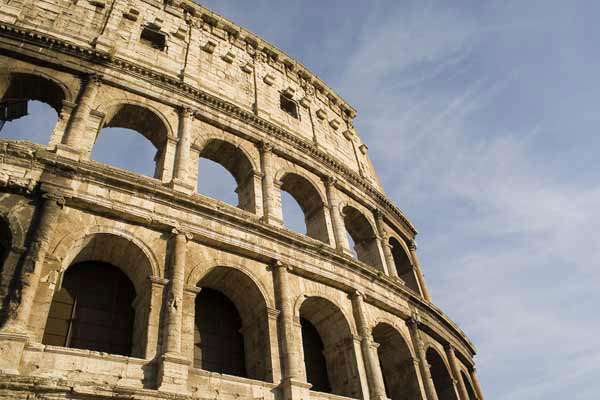
\includegraphics[width=0.6\textwidth]{exam-cover-05}

  \vspace{5mm}

  \textbf{\Huge{Level Three Calculus}}

  \vspace{2mm}

  \textbf{\Huge{Differentiation}}
\end{center}

\vspace{5mm}

\noindent
\large{There are three questions, worth a total of \numpoints\ marks.\\
       Attempt ALL questions, showing all working.\\
       Read questions carefully before attempting them.\\
       Marks are available for partial answers.\\
       The amount of time expected to be spent per question may not necessarily correlate ``nicely'' to the number of marks.\\
       Diagrams may be used to support answers.\\
       Candidates who do not provide diagrams for some questions may be disadvantaged.\\
       Some marks are given for clarity and neatness of solutions or proofs.}
\vspace{2mm}

\begin{tabular}{ll}
  \textbf{Time Allowed:}& One Hour\\
  \textbf{Achieved:}& 11 marks\\
  \textbf{Merit:}& 19 marks\\
  \textbf{Excellence:}& 27 marks
\end{tabular}

\vfill

\begin{center}
  \gradetable[h][questions]
  \vspace{2mm}

  \textbf{Available Grades:} \textit{Not Achieved}\quad\textit{Achieved}\quad\textit{Merit}\quad\textit{Excellence}
\end{center}

\end{coverpages}

\begin{questions}
  \question
    \begin{parts}
      \part For i. and ii., find the derivatives of the given functions with respect to $ x $.
        \begin{subparts}
          \subpart[1] $ f(x) = e^{-\sqrt{x}} $
          \subpart[1] $ g(x) = \dfrac{2 \sqrt[3]{x + 1}}{\ln x} $
        \end{subparts}

      \part The path through space of a particle can be modelled by the following 2D parametric equation.
            \begin{align*}
                x(t) &= \sin(2t)\\
                y(t) &= \sin(t + \sin(2t))
            \end{align*}
      \begin{subparts}
        \subpart[3] Calculate the velocity of the particle as it passes through the origin at $ t = 0 $. Give your answer
                  in the form $ (v_x(t), v_y(t)) $, where $ v_x(t) $ and $ v_y(t) $ are the $ x $ and $ y $ components
                  of the velocity respectively.
        \subpart[3] Write down an expression for $ \od{y}{x} $, and explain its geometric interpretation.
      \end{subparts}
    \end{parts}
  \question
    \begin{parts}
      \part[3] Find the equation of the tangent line to the curve
            \begin{displaymath}
              y^5 + 4x^2y - x^3 + 2x^3y - 1 = 0
            \end{displaymath}
            at the point $ (-5, 1) $. \textit{Write your answer in the form $ y = mx + c $.}
      \part Amanda is dreaming that water is leaking out of a tank shaped like an upside-down cone, as in figure \ref{fig:cone}. The radius
            of the base of the cone is $ R = \SI{2}{\metre} $, and the height of the cone is $ H = \SI{5}{\metre} $.
            \begin{figure}
              \centering
              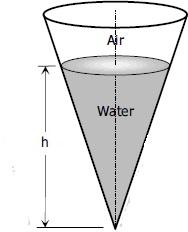
\includegraphics[width=0.2\textwidth]{conical}
              \caption{The leaky tank.\label{fig:cone}}
            \end{figure}
        \begin{subparts}
          \subpart[3] Water is leaking out of the tank at a constant rate of \SI{0.2}{\metre\cubed} per second. What is the rate-of-change of the
                   depth of the water at the instant that the depth of the water is $ h = \SI{3}{\metre} $?
          \subpart[2] Amanda notices that the tank has less water in it than she would prefer, and dreams that she begins to
                   pump water back in at a constant rate \textbf{without plugging the original leak}. When the height of
                   the water is $ h = \SI{2}{\metre} $, the water level is rising at a rate of $ \SI{0.1}{\metre\per\second} $.
                   Find the rate at which water is being pumped back in.
        \end{subparts}
    \end{parts}
  \question
    \begin{parts}
      \part[2] Let $ \varphi(x) = \sqrt{x} $. Explain why the limit $ \lim_{x \to 0} \varphi(x) $ does not exist, even
            though $ \varphi(x) $ has a value at $ x = 0 $.
      \part[3] Recall that an isoceles triangle is a triangle with two equal sides. Find the side-lengths of the isoceles
            triangle of greatest area with perimeter $ P $.
      \part[3] Peter Pan is opening a lemonade stand in Taumarunui. Each lemon costs \$5, but only half a lemon is needed
            for each glass; there is also an initial fixed cost of \$5 for the glasses, sugar, and other equipment.
            After conducting a survey, Peter finds that if he sells the lemonade at a price $ c $
            per glass, the expected demand is $ D = 30e^{-c/2} $. What price should he sell a glass for in order
            to maximise his profit?
    \end{parts}
\end{questions}
\end{document}
